% -----------------------------------------------
% TISMIR / ISMIR 2026 Paper — GTZAN-Probe
% -----------------------------------------------

\documentclass{article}
\usepackage[T1]{fontenc}
\usepackage[utf8]{inputenc}
\usepackage[submission]{ismir}
\usepackage{amsmath,cite,url}
\usepackage{graphicx}
\usepackage{color}
\usepackage{booktabs}
\usepackage{multirow}
\usepackage{xspace}
\usepackage{placeins}

\title{Probing What Music Classifiers Actually Learn:\\ A Multi-Method Explainability Analysis of Genre Classification on GTZAN}

\oneauthor
  {Anonymous Author}
  {Anonymous Affiliation\\\texttt{anonymous@ismir.net}}

\def\authorname{J. Abimbola}

\sloppy

\begin{document}

\maketitle

\begin{abstract}
Convolutional neural networks (CNNs) achieve competitive accuracy on music genre classification, yet it remains unclear whether their decisions are grounded in musically meaningful features or in dataset artifacts such as recording noise, silence patterns, and artist fingerprints. This paper presents a systematic, multi-method explainability analysis of a CNN trained on the GTZAN dataset, using SHapley Additive exPlanations (SHAP), Local Interpretable Model-agnostic Explanations (LIME), and complementary attention visualisation from a fine-tuned Audio Spectrogram Transformer (AST). We introduce a four-metric evaluation framework comprising music-informed spectral alignment, faithfulness under perturbation, inter-method agreement, and artifact-focused attribution ratios. Results show strong genre dependence: some classes (notably hip-hop) exhibit attribution patterns consistent with expected low-frequency cues, while others show elevated attribution in non-musical regions (e.g., silence), consistent with potential shortcut use. SHAP and LIME also exhibit systematically low agreement for the same predictions, indicating strong method dependence of explanatory narratives. Overall, the study supports multi-method triangulation and conservative, domain-aware interpretation of explainable artificial intelligence (XAI) outputs in music information retrieval (MIR).
\end{abstract}

\section{Introduction}\label{sec:introduction}

Music genre classification has served as a foundational benchmark in music information retrieval since the seminal work of Tzanetakis and Cook \cite{Tzanetakis2002}. Over the past decade, deep learning models operating on mel spectrogram representations have driven classification accuracy on the GTZAN benchmark to near-perfect levels. Recent architectures, including capsule neural networks with aggressive data augmentation, have reported accuracies as high as 99.9\% \cite{Lim2025}, and other deep architectures have independently exceeded 99\% \cite{Nanni2023}, suggesting that the problem is approaching saturation on this benchmark. In terms of raw classification performance, there is little room left to gain.

Yet this apparent ceiling of discovery masks a more fundamental and largely unresolved question: what are these models actually learning? High classification accuracy on GTZAN does not necessarily indicate that a model has internalized meaningful musical characteristics such as rhythm, harmony, or timbre. Prior work has demonstrated that classifiers may instead exploit dataset-specific artifacts, including recording conditions, duplicate clips, and labeling inconsistencies, to achieve high scores while failing to capture genuine genre semantics \cite{Sturm2016, sturm2013gtzan}. A model that achieves 99\% accuracy by recognizing microphone characteristics is fundamentally different from one that has learned the 12-bar blues structure or the sub-bass patterns of hip-hop, even though their test metrics may be identical. The research frontier, therefore, has shifted from improving accuracy to interrogating the nature of what is learned.

This distinction is not merely academic. In MIR, models are increasingly deployed in production systems for recommendation, cataloguing, and rights management \cite{Fu2011}. If these systems base decisions on spurious correlations (microphone characteristics, compression artifacts, or silence padding), performance can degrade when deployment data does not share those incidental properties \cite{Geirhos2020,Lapuschkin2019}. The field of eXplainable Artificial Intelligence (XAI) \cite{Arrieta2020} offers tools to interrogate model decisions, yet rigorous XAI evaluation remains comparatively limited in MIR relative to broader ML subfields.

Prior work on explainability in music classification remains relatively sparse and methodologically focused on single-method case studies. Mishra et~al. \cite{Mishra2017} applied LIME to music content analysis but did not validate whether the identified regions corresponded to musically meaningful features. Haunschmid et~al. \cite{Haunschmid2020} proposed audioLIME with source-separation-based explanations, advancing interpretability but not systematically evaluating faithfulness or cross-method consistency. To our knowledge, prior MIR studies have not commonly combined multiple complementary XAI techniques with explicit domain-informed priors and quantitative faithfulness testing in one unified evaluation pipeline.

The GTZAN dataset \cite{Tzanetakis2002} presents a particularly instructive test case. Despite being the most widely used benchmark in genre classification, GTZAN contains well-documented flaws: artist repetition within genres, inconsistent recording quality across genres, and faulty or mislabelled clips \cite{sturm2013gtzan}. These flaws are not merely a limitation; they serve as a natural instrument for probing whether classifiers learn music or metadata. As Sturm \cite{Sturm2014} argued, a genre classifier may function as a "horse", a system that exploits dataset regularities without learning the intended concept.

This paper addresses the following research questions:

\begin{enumerate}
\item[\textbf{RQ1}:] To what extent do CNN-based genre classifiers attend to musicologically meaningful spectral features versus dataset artifacts?
\item[\textbf{RQ2}:] Do different XAI methods (SHAP, LIME, attention) provide consistent explanations for the same model decisions?
\item[\textbf{RQ3}:] Can genuine musicological learning be quantitatively distinguished from spurious correlation exploitation?
\end{enumerate}

The contributions of this paper are as follows:  a multi-method explainability pipeline combining SHAP and LIME for a common CNN classifier, with AST attention used as an auxiliary qualitative perspective;  a four-metric quantitative framework for explanation assessment; evidence of genre-dependent differences in whether attributions align with music-informed spectral expectations or artifact-sensitive regions; and a demonstration that XAI method choice substantially affects explanatory conclusions, motivating multi-method triangulation as standard practice.

\section{Related Work}\label{sec:related}

\subsection{Music genre classification}

Music genre classification has been a central task in music information retrieval (MIR) since the pioneering work of Tzanetakis and Cook \cite{Tzanetakis2002}, which introduced a feature-based approach using timbral texture, rhythmic content, and pitch features. Early systems relied on handcrafted descriptors such as MFCCs, spectral centroid, zero-crossing rate, and beat histograms, combined with classical classifiers including k-nearest neighbours and support vector machines \cite{Li2003}.

The field has since shifted toward deep learning approaches that learn representations directly from audio. Convolutional neural networks (CNNs) operating on mel spectrograms have become the dominant paradigm, demonstrating strong performance across multiple MIR tasks \cite{Dieleman2014, Choi2017}. Variants incorporating residual connections, attention mechanisms, and multi-scale feature extraction have further improved performance \cite{Palanisamy2020}. More recently, Transformer-based architectures such as the Audio Spectrogram Transformer (AST) \cite{Gong2021} and large-scale self-supervised models like MERT \cite{Li2024} have pushed performance closer to saturation by leveraging large pre-training corpora.

Despite these advances, performance gains on GTZAN have plateaued, with multiple studies reporting accuracies exceeding 95\% and, in some cases, approaching 100\% \cite{Lim2025,Nanni2023}. This saturation raises questions about whether further improvements reflect genuine advances in musical understanding or exploitation of dataset-specific regularities \cite{Sturm2016}.

\subsection{GTZAN dataset critique and shortcut learning}

The GTZAN dataset \cite{Tzanetakis2002}, while widely used, has been extensively criticised for its structural flaws. Sturm \cite{sturm2013gtzan} conducted a comprehensive audit, identifying duplicate recordings, mislabelled tracks, and substantial artist overlap between training and test sets. These issues introduce confounding factors that allow models to achieve artificially high performance without learning meaningful genre characteristics.

This phenomenon is closely related to the concept of \textit{shortcut learning}, where models exploit spurious correlations that are predictive in the training data but not causally related to the task \cite{Geirhos2020}. In the context of GTZAN, such shortcuts may include recording conditions, production styles, or artist-specific characteristics rather than genre-defining musical features. Sturm \cite{Sturm2014} characterised this issue through the ``horse'' analogy, highlighting that classifiers may appear successful while relying on unintended cues.

Subsequent work has reinforced these concerns by demonstrating that simple baselines exploiting metadata or recording artifacts can achieve competitive performance \cite{Flexer2007}. More broadly, the problem of dataset bias and spurious correlations has been widely studied in machine learning, with implications for model robustness and generalisation \cite{Torralba2011}. These findings motivate the need for methods that go beyond accuracy to interrogate what models actually learn.

\subsection{Explainability in MIR}

Explainable Artificial Intelligence (XAI) has emerged as a critical tool for understanding model behaviour, particularly in domains where interpretability and trust are essential \cite{Arrieta2020}. In MIR, however, the application of XAI remains less extensive than in computer vision and natural language processing, where method development and benchmarking are more mature.

Early work by Mishra et~al.\ \cite{Mishra2017} applied LIME \cite{Ribeiro2016} to music content analysis, demonstrating that perturbation-based explanations can highlight salient spectrogram regions. Haunschmid et~al.\ \cite{Haunschmid2020} proposed audioLIME, which improves upon standard LIME by generating perturbations through source separation, yielding more musically meaningful explanations. Gradient-based attribution methods, including saliency maps and Grad-CAM \cite{Selvaraju2017}, have also been applied to audio classification tasks, though often without rigorous validation against domain knowledge.

More recently, attention-based models such as AST \cite{Gong2021} have been used to provide interpretability through attention visualisation. However, the extent to which attention weights correspond to causal feature importance remains debated \cite{Jain2019}. More broadly, the XAI literature has shown that explanation methods can disagree or fail basic reliability checks, motivating multi-method validation rather than reliance on a single technique \cite{Krishna2022,Adebayo2018}.

\subsection{Evaluating explanations and the disagreement problem}

A central challenge in XAI is the evaluation of explanation quality. Metrics such as faithfulness, sensitivity, and robustness have been proposed to assess whether explanations accurately reflect model decision processes \cite{Samek2017, Hooker2019}. In MIR practice, many studies still emphasise qualitative inspection, with fewer works reporting systematic quantitative explanation diagnostics \cite{Mishra2017,Haunschmid2020}.

Another critical issue is the \textit{disagreement problem}: different XAI methods often produce substantially different explanations for the same prediction \cite{Krishna2022}. This has been observed across domains and raises concerns about the reliability of individual explanation techniques. In audio and MIR contexts, where perceptual structure is complex and multi-dimensional, this issue can be particularly challenging to interpret.

Despite these challenges, there is still limited MIR work that simultaneously applies multiple complementary XAI methods to the same model, quantitatively evaluates explanation quality, and grounds explanations in domain-specific (musicological) expectations. This paper addresses that gap by introducing a multi-method, quantitatively validated framework for analysing what genre classifiers learn on GTZAN.

\section{Methodology}\label{sec:methodology}

\subsection{Dataset and pre-processing}\label{subsec:dataset}

The GTZAN dataset \cite{Tzanetakis2002} is used, comprising 1,000 audio clips of 30 seconds each, distributed equally across 10 genres: blues, classical, country, disco, hip-hop, jazz, metal, pop, reggae, and rock. Following the audit methodology of Sturm \cite{sturm2013gtzan}, known faulty clips (exact duplicates, severely distorted recordings, and mislabelled tracks) are flagged and excluded: 4 duplicates, 2 corrupt recordings, and 2 mislabelled clips are removed, restricting the analysis to the remaining 992 clean clips.

Audio is loaded at 22,050~Hz, the standard sample rate adopted across MIR research \cite{Tzanetakis2002,McFee2015}. This rate captures the full perceptually relevant audio spectrum up to its 11,025~Hz Nyquist limit while halving storage and computation relative to CD-quality 44,100~Hz. Mel spectrograms are computed via librosa \cite{McFee2015} using a 2,048-sample DFT window ($\approx$93~ms at 22,050~Hz) and a 512-sample hop length ($\approx$23~ms; 75\% frame overlap). The window length balances frequency resolution ($\approx$10.8~Hz per bin, sufficient to differentiate harmonic partials) against temporal smearing, and these parameters follow established conventions for spectrogram-based music classification \cite{Dieleman2014,Choi2017}. A filterbank of 128 mel-spaced bins is used: the mel scale approximates the auditory system's critical-band spacing, and 128 bins is the predominant choice in the literature for balancing perceptual coverage against feature dimensionality \cite{Choi2017,McFee2015}.

For the CNN, 3-second segments are randomly cropped from each 30-second clip during training. This duration serves a dual purpose. First, at the above settings a 3-second window produces approximately 129 time frames, yielding a near-square spectrogram that, after a minor resize to $128 \times 128$ pixels, matches the mel-bin count and is directly compatible with standard square-input convolutional architectures without distorting the time-frequency aspect ratio \cite{Dieleman2014}. Second, 3 seconds spans roughly three to six beats at typical genre tempi (60--120~BPM), providing enough context to capture the rhythmic periodicity and timbral texture that underpin genre identity \cite{Tzanetakis2002}. Randomly cropping segments from the full 30-second clip increases the effective number of training samples, serving as an implicit form of data augmentation that mitigates overfitting on the relatively small 992-clip dataset—conceptually similar to the time-masking approach used in SpecAugment \cite{Park2019}. Spectrograms are converted to log-mel scale before input; the logarithric compression aligns the energy representation with the auditory system's approximately logarithmic loudness sensitivity and stabilises the dynamic range across genre styles.

For the AST, 10-second segments are used and audio is resampled to 16,000~Hz. Both choices directly match the pre-training configuration of the AST model \cite{Gong2021}: the original model was pre-trained on AudioSet using 10-second clips at 16,000~Hz, and deviating from these settings would introduce a distributional mismatch between the pre-trained patch embeddings and the fine-tuning inputs, degrading transfer efficiency.

The dataset is split into 80\% training and 20\% evaluation sets using stratified sampling to ensure balanced genre representation, yielding approximately 794 training and 198 evaluation clips. The evaluation partition serves a dual role: it is used as a per-epoch validation set during training while monitoring validation loss and accuracy at every epoch and checkpointing the model at peak validation accuracy. The validation set is also the test set and no further separate test set partition is created given the limited corpus size; this design is a known constraint of single-split evaluation on small datasets \cite{Flexer2007}, and its implications for result interpretation are discussed in Section~\ref{sec:discussion}.

\subsection{CNN architecture (MusicCNN)}\label{subsec:cnn}

The model is a purpose-built CNN designed for interpretability research. The architecture consists of three convolutional blocks, each containing two $3 \times 3$ convolutional layers with batch normalisation \cite{Ioffe2015}, ReLU activation, $2 \times 2$ max pooling, and spatial dropout (rate 0.15). Channel dimensions progress as $1 \rightarrow 32 \rightarrow 64 \rightarrow 128$. An adaptive average pooling layer produces $4 \times 4$ spatial features, followed by a two-layer fully connected head ($2{,}048 \rightarrow 256 \rightarrow 10$) with dropout (rate 0.4). The model totals approximately 814K parameters.

Residual connections and complex skip pathways are deliberately avoided to ensure that feature attribution methods can trace contributions through the network without ambiguity. This design choice prioritises interpretability over raw performance.

Training employs the AdamW optimiser \cite{Kingma2015} with an initial learning rate of $10^{-3}$, cosine annealing schedule with linear warmup \cite{Loshchilov2017}, and cross-entropy loss with label smoothing of 0.1. Data augmentation includes SpecAugment \cite{Park2019} (frequency and time masking) and mixup \cite{Zhang2018} ($\alpha = 0.3$). Training proceeds for 120 epochs with a batch size of 32. All experiments use PyTorch \cite{Paszke2019} on Apple MPS (Metal Performance Shaders) hardware acceleration.

\subsection{Explainability methods}\label{subsec:xai_methods}

Three complementary XAI techniques are applied, each grounded in different theoretical assumptions:

\subsubsection{SHAP (SHapley Additive exPlanations)}

SHAP \cite{Lundberg2017} is rooted in cooperative game theory, assigning each input feature an importance value based on Shapley values \cite{Shapley1953}. The DeepExplainer variant is employed, using a background distribution of 50 stratified training spectrograms (5 per genre) to compute expected model behaviour. For each correctly classified test clip, SHAP produces a $128 \times 128$ attribution map indicating how each mel spectrogram bin contributed to the predicted class.

SHAP offers theoretical guarantees of local accuracy, missingness, and consistency that other attribution methods lack. However, the gradient-based approximation in DeepExplainer introduces some approximation error, and the method operates at the individual pixel level without awareness of perceptual grouping.

\subsubsection{LIME (Local Interpretable Model-agnostic Explanations)}

LIME \cite{Ribeiro2016} treats the model as a black box, perturbing the input and observing output changes to fit a local interpretable surrogate model. Each mel spectrogram is segmented into superpixels using Simple Linear Iterative Clustering (SLIC) \cite{Achanta2012}, 1,000 perturbations are generated by randomly masking subsets of superpixels, and a weighted Ridge regression model is fitted to approximate the local decision boundary.

Unlike SHAP, LIME operates at the superpixel level, producing coarser attributions. Its model-agnostic nature means it can be applied to any classifier without access to gradients. We note that SLIC was designed for natural images; when applied to spectrograms it may not preserve perceptual time-frequency structure, so LIME outputs are interpreted as local sensitivity summaries rather than direct perceptual parts.

\subsubsection{AST attention maps}

As a third perspective, an Audio Spectrogram Transformer (AST) \cite{Gong2021} pre-trained on AudioSet is fine-tuned and CLS token attention weights are extracted from the final self-attention layer. The AST processes each audio clip as a sequence of overlapping $16 \times 16$ spectrogram patches, and the CLS token's attention distribution indicates which patches the model attends to when making its classification decision.

A two-phase fine-tuning strategy is employed: 10 epochs of linear probing (frozen backbone, trained head only) followed by 20 epochs of full fine-tuning with a reduced learning rate ($10^{-5}$). Cross-entropy loss with label smoothing of 0.1 is used throughout.

The known caveat that attention weights do not necessarily reflect causal importance \cite{Jain2019} is acknowledged. Accordingly, AST attention is used only as a qualitative auxiliary signal and is not included in the quantitative SHAP--LIME agreement statistics.

\subsection{Quantitative validation framework}\label{subsec:validation}

A central contribution of this work is a four-metric framework for evaluating explanation quality in the context of music classification:

\subsubsection{Music-informed spectral alignment ($\rho_{\text{align}}$)}

Expected frequency-band importance rankings are defined per genre as a hypothesis-driven prior informed by MIR literature on timbre/spectral cues \cite{Tzanetakis2002,Fu2011}, not as objective ``ground truth.'' Five broad bands are considered: sub-bass (0--60~Hz), bass (60--250~Hz), mid (250--2,000~Hz), upper-mid (2,000--6,000~Hz), and brilliance (6,000--20,000~Hz). For each genre, we specify an expected ranking (e.g., hip-hop prioritising low bands, classical prioritising upper-mid/brilliance), then test whether observed attributions follow this prior.

For each genre, the mean absolute SHAP value within each frequency band is computed, these bands are ranked by attribution magnitude, and the Spearman rank correlation ($\rho$) between the observed and expected rankings is computed:

\begin{equation}\label{eq:alignment}
\rho_{\text{align}} = 1 - \frac{6 \sum_{i=1}^{n} d_i^2}{n(n^2 - 1)}
\end{equation}

\noindent where $d_i$ is the rank difference for band $i$ and $n = 5$ is the number of frequency bands. Values near $+1$ indicate agreement with the prior; values near $-1$ indicate inverse ranking. Because $n$ is small, we treat $\rho_{\text{align}}$ primarily as an effect-size descriptor.

\subsubsection{Faithfulness}

Faithfulness measures whether the identified important regions are genuinely used by the model. We follow the occlusion protocol of Samek et~al.\ \cite{Samek2017} and Hooker et~al.\ \cite{Hooker2019}: for each explained clip, we progressively mask the top-$k$\% of pixels (by SHAP magnitude) with zeros and measure the drop in prediction confidence:

\begin{equation}\label{eq:faithfulness}
\text{Faith}(k) = P(\hat{y} \mid \mathbf{x}) - P(\hat{y} \mid \mathbf{x}_{\setminus \text{top-}k})
\end{equation}

\noindent where $\hat{y}$ denotes the model's predicted class for input $\mathbf{x}$, $P(\hat{y} \mid \mathbf{x})$ is the original confidence, and $P(\hat{y} \mid \mathbf{x}_{\setminus \text{top-}k})$ is the confidence after masking. A large drop confirms that SHAP correctly identified decision-critical regions. We evaluate at $k \in \{5, 10, 20, 30, 50\}\%$.

\subsubsection{Inter-method agreement}

To quantify the disagreement problem \cite{Krishna2022}, we compute three agreement metrics between SHAP and LIME attribution maps: Pearson correlation coefficient $r$, Spearman rank correlation $\rho$, and intersection-over-union (IoU) of the top-10\% most important pixels:

\begin{equation}\label{eq:iou}
\text{IoU}_{10} = \frac{|\mathcal{S}_{10}^{\text{SHAP}} \cap \mathcal{S}_{10}^{\text{LIME}}|}{|\mathcal{S}_{10}^{\text{SHAP}} \cup \mathcal{S}_{10}^{\text{LIME}}|}
\end{equation}

\noindent where $\mathcal{S}_{10}^{\text{SHAP}}$ and $\mathcal{S}_{10}^{\text{LIME}}$ are the sets of pixels in the top 10\% attribution magnitude under SHAP and LIME, respectively.

\subsubsection{Spurious correlation detection}

We compare SHAP attributions in spectrogram regions likely to contain artifacts versus regions containing musical content. Two ratios are computed: (1) the silence ratio, comparing mean SHAP magnitude in low-energy (silence) bins to high-energy bins; and (2) the edge ratio, comparing SHAP in temporal edge regions (first/last 10\% of the spectrogram) to centre regions. A silence ratio exceeding 1.0 indicates the model assigns more importance to silence than to musical content, which is a strong indicator of artifact exploitation.

\subsubsection{Statistical interpretation}

Our per-genre alignment uses rankings over only five frequency bands. We therefore avoid strong null-hypothesis claims from $p$-values and emphasise effect sizes, cross-metric consistency, and qualitative inspection. In addition, we report bootstrap confidence intervals for global summary metrics (genre-resampled; 2,000 draws), including alignment, agreement, and faithfulness aggregates. Conclusions are phrased as evidence ``consistent with'' potential shortcut use rather than causal proof.

\section{Results}\label{sec:results}

\subsection{Classification performance}\label{subsec:classification}

It should be noted that maximising classification accuracy is not the objective of this work. The model is designed to achieve sufficient task competence that its decisions are meaningful and worth explaining, not to compete with state-of-the-art classifiers. An accuracy level well above chance but below saturation is, in fact, preferable for explainability research: a model that struggles on some genres reveals the limits and biases of its learned representations more clearly than one that classifies everything perfectly \cite{Sturm2016}.

The MusicCNN achieves an overall test accuracy of 83.4\% on 198 test clips. Classical and jazz are classified perfectly (100\%), while disco and rock prove most challenging (65\%). These confusion patterns align with musicological similarity: disco and rock share similar rhythmic drive and spectral energy distributions, while classical and jazz have highly distinctive timbral profiles.

The full confusion structure is shown in \figref{fig:confusion_matrix}. The largest error cluster occurs between rock and pop (7 total: 6 rock clips predicted as pop, 1 pop clip predicted as rock), followed by country and rock (4 total: 3 country clips predicted as rock, 1 rock clip predicted as country), and disco and pop (3 total, all in the disco$\rightarrow$pop direction). These confusions are largely asymmetric and provide meaningful targets for XAI interrogation: understanding \textit{why} the model preferentially maps rock to pop, rather than the reverse, may reveal whether it has learned the relevant distinguishing features or is exploiting shared spectral characteristics.


\begin{figure*}[!t]
  \centering
  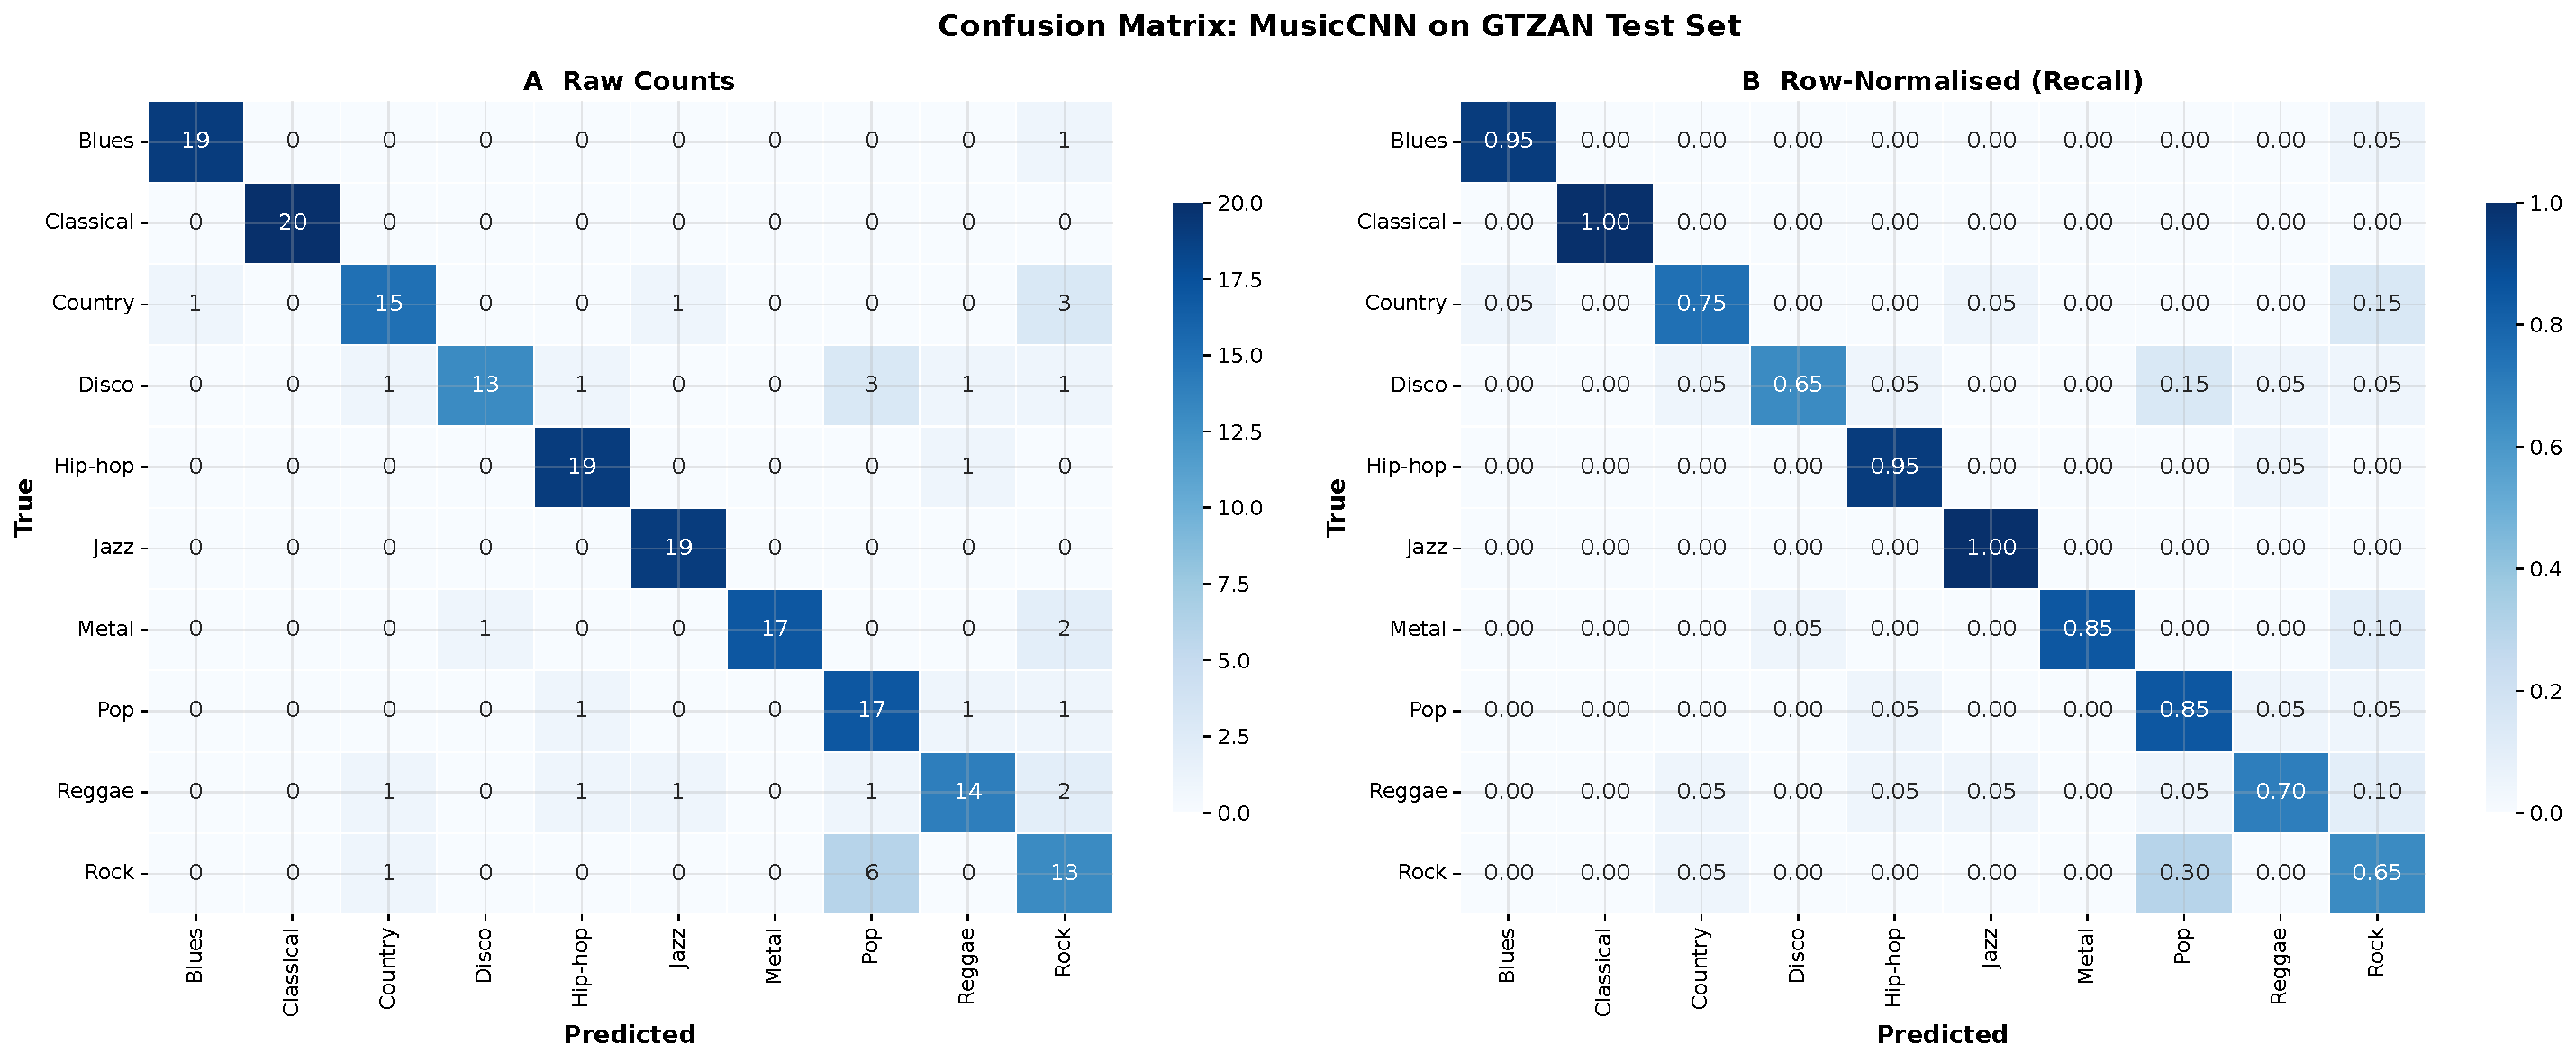
\includegraphics[alt={Confusion matrix showing classification results across 10 genres},width=0.72\textwidth]{02_confusion_matrix.pdf}
  \caption{Confusion matrix for MusicCNN on the GTZAN test set. Classical and jazz show perfect separation; pop and rock exhibit the highest mutual confusion.}
  \label{fig:confusion_matrix}
\end{figure*}

\subsection{SHAP explanations}\label{subsec:shap_results}

SHAP attribution overlays for representative correctly classified clips are presented in \figref{fig:shap_gallery}. The overlays reveal qualitatively distinct attribution patterns across genres. Classical clips show distributed high-frequency attribution consistent with orchestral overtone richness. Hip-hop shows concentrated low-frequency attribution aligned with bass-heavy production. Jazz exhibits broad spectral attribution reflecting harmonic complexity.

\begin{figure*}[!t]
  \centering
  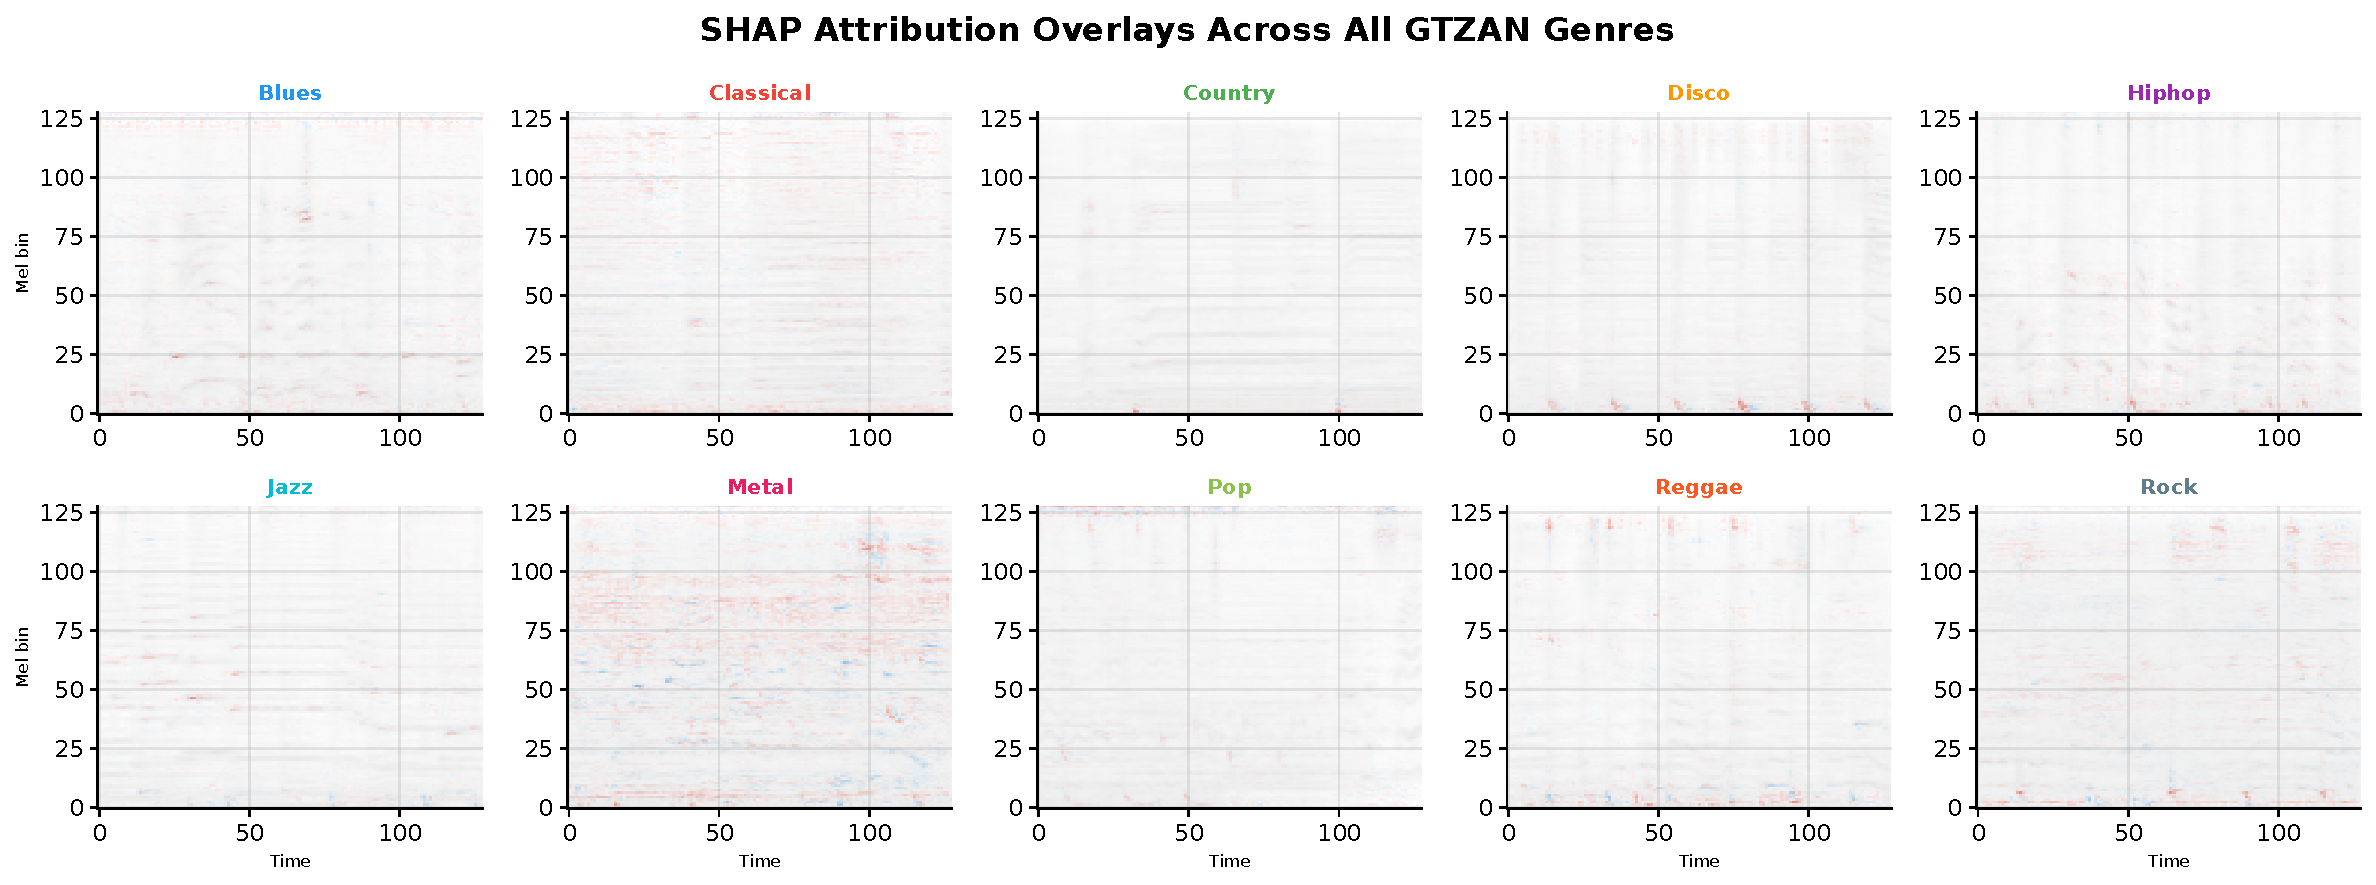
\includegraphics[alt={Gallery of SHAP attribution overlays on mel spectrograms for ten genres},width=0.95\textwidth]{FINAL_01_shap_hero.pdf}
  \caption{SHAP attribution overlays on mel spectrograms for correctly classified clips from each genre. Red indicates positive attribution (pushes toward the predicted class); blue indicates negative attribution.}
  \label{fig:shap_gallery}
\end{figure*}

Aggregated SHAP attributions by frequency band are shown in \figref{fig:shap_bands}. Notable patterns include the dominance of low-frequency bands for hip-hop and reggae, mid-range salience for country and rock, and high-frequency emphasis for classical and metal.

\begin{figure*}[!t]
  \centering
  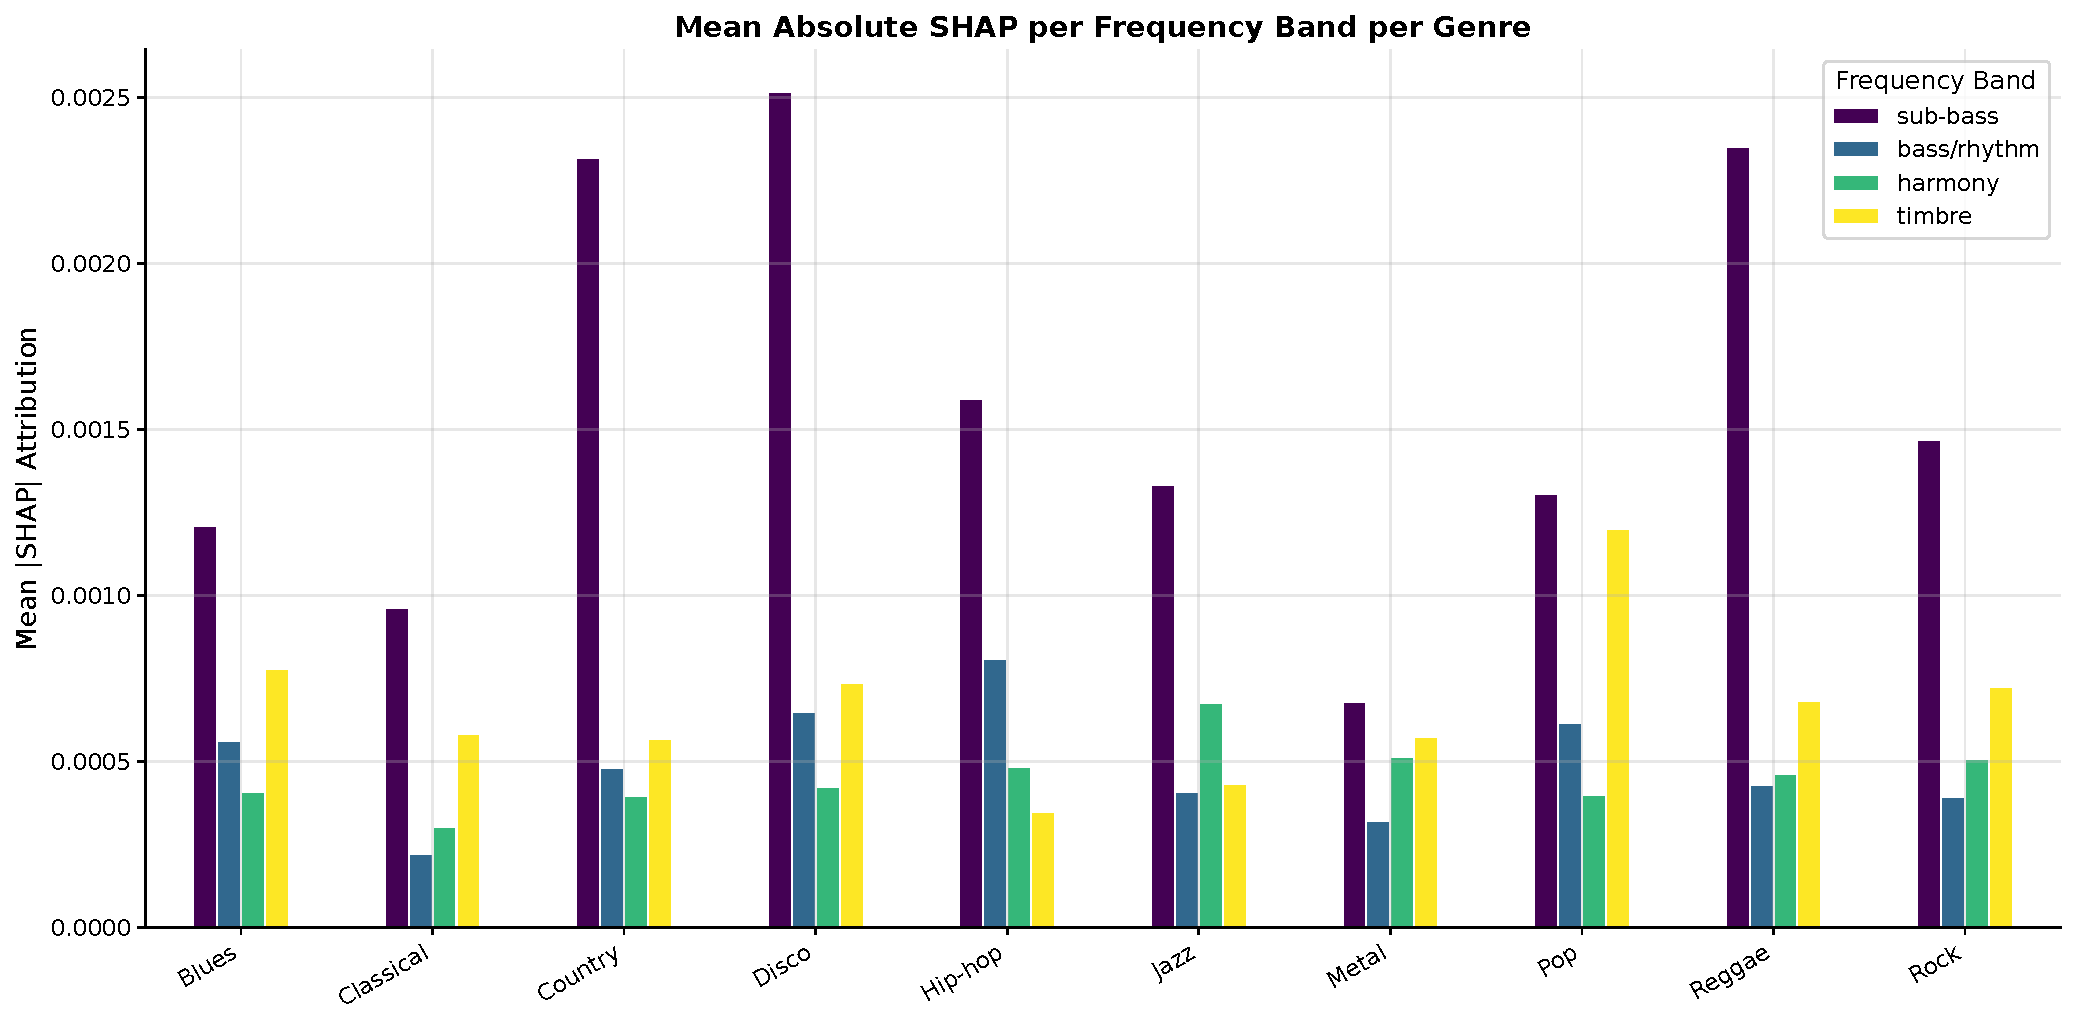
\includegraphics[alt={Bar chart showing mean absolute SHAP attribution per frequency band per genre},width=0.95\textwidth]{03_shap_frequency_bands.pdf}
  \caption{Mean absolute SHAP attribution per frequency band per genre, revealing genre-specific spectral attention patterns.}
  \label{fig:shap_bands}
\end{figure*}

\subsection{LIME explanations}\label{subsec:lime_results}

LIME superpixel explanations for the same clips are shown in \figref{fig:lime_gallery}. LIME identifies broader contiguous regions compared to SHAP's pixel-level attributions, reflecting the superpixel granularity of the perturbation scheme.

\begin{figure*}[!t]
  \centering
  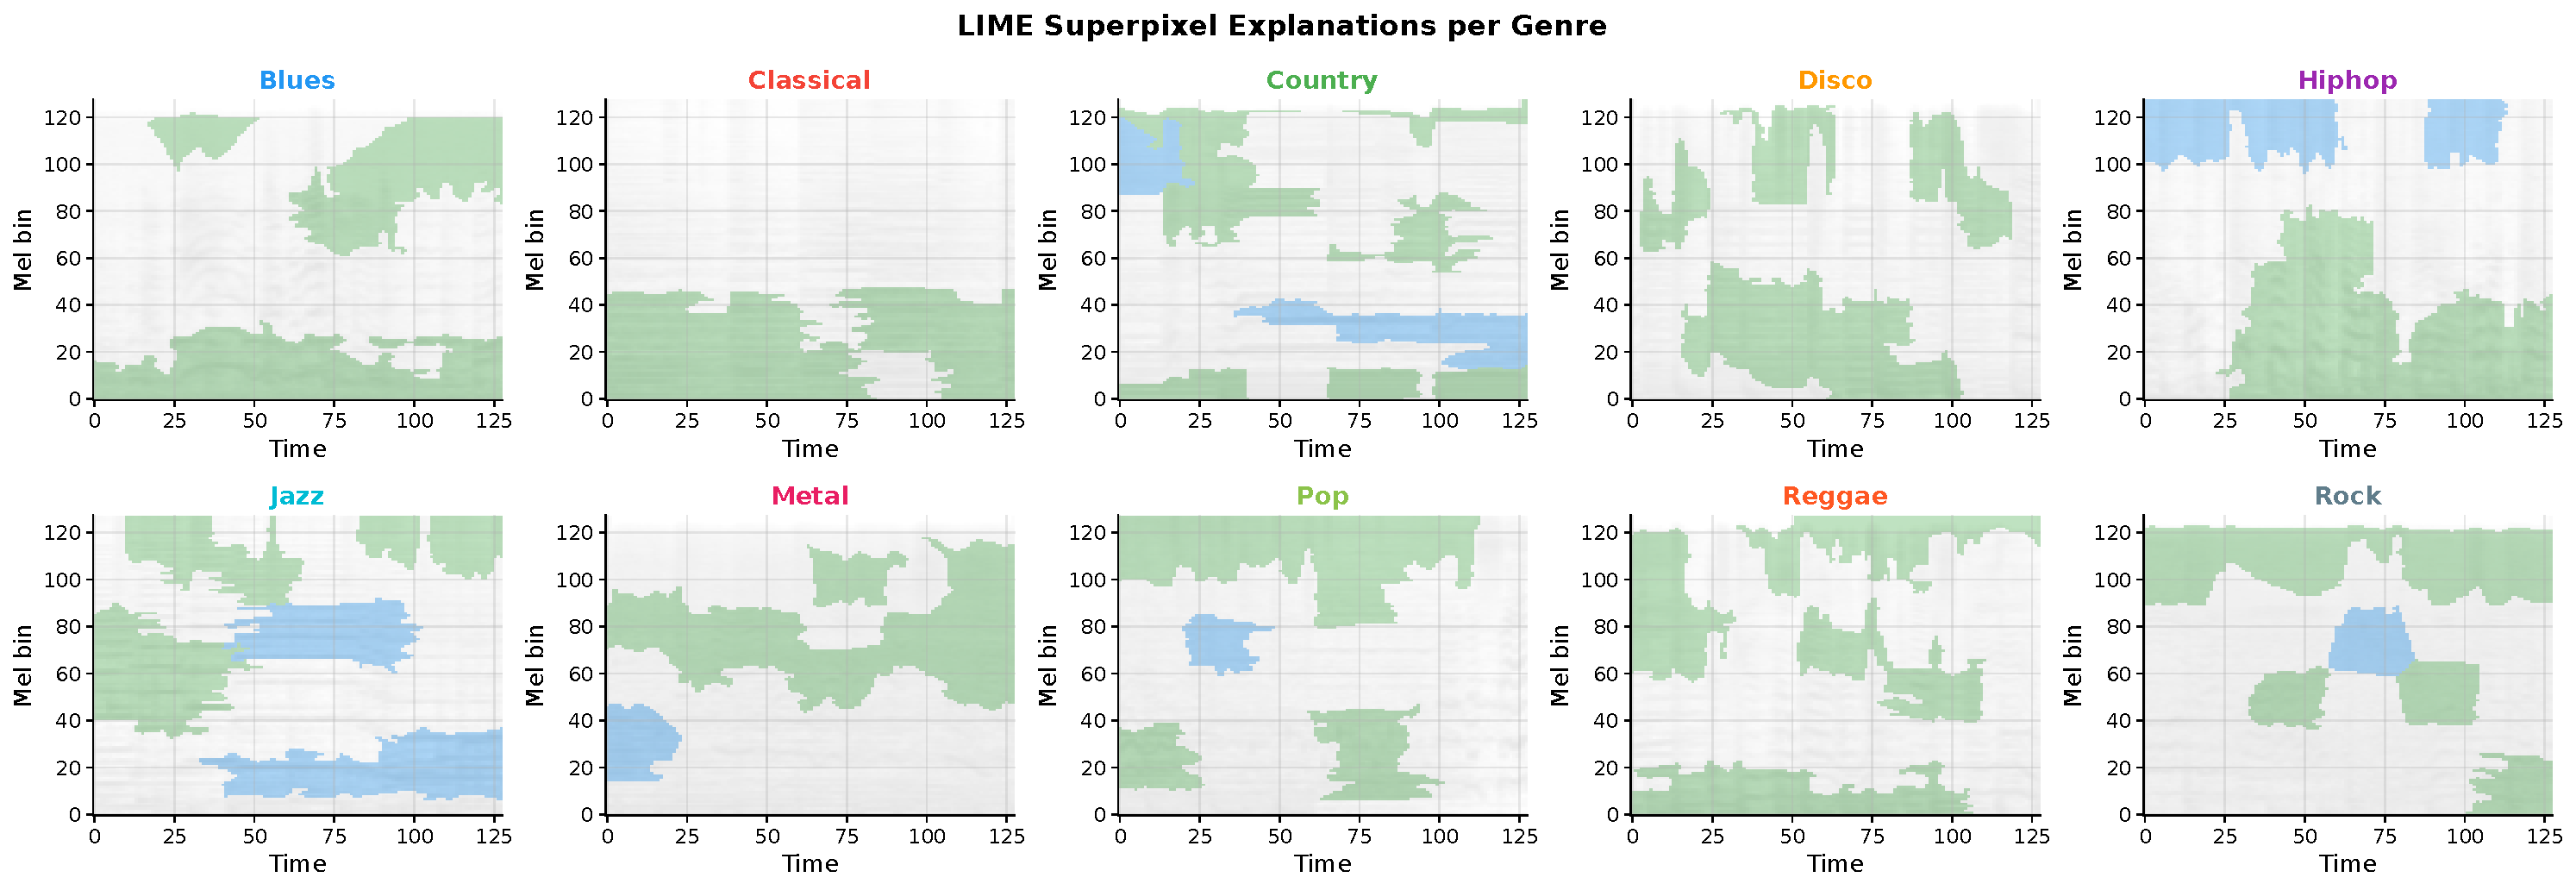
\includegraphics[alt={Gallery of LIME superpixel explanations for ten genres},width=0.95\textwidth]{04_lime_gallery.pdf}
  \caption{LIME superpixel importance maps for correctly classified clips. Green regions indicate positive contribution to the predicted genre; red indicates negative contribution.}
  \label{fig:lime_gallery}
\end{figure*}

A consolidated view of all four quantitative XAI metrics discussed in the following subsections is provided in \figref{fig:quantitative_panel}.

\begin{figure*}[!t]
  \centering
  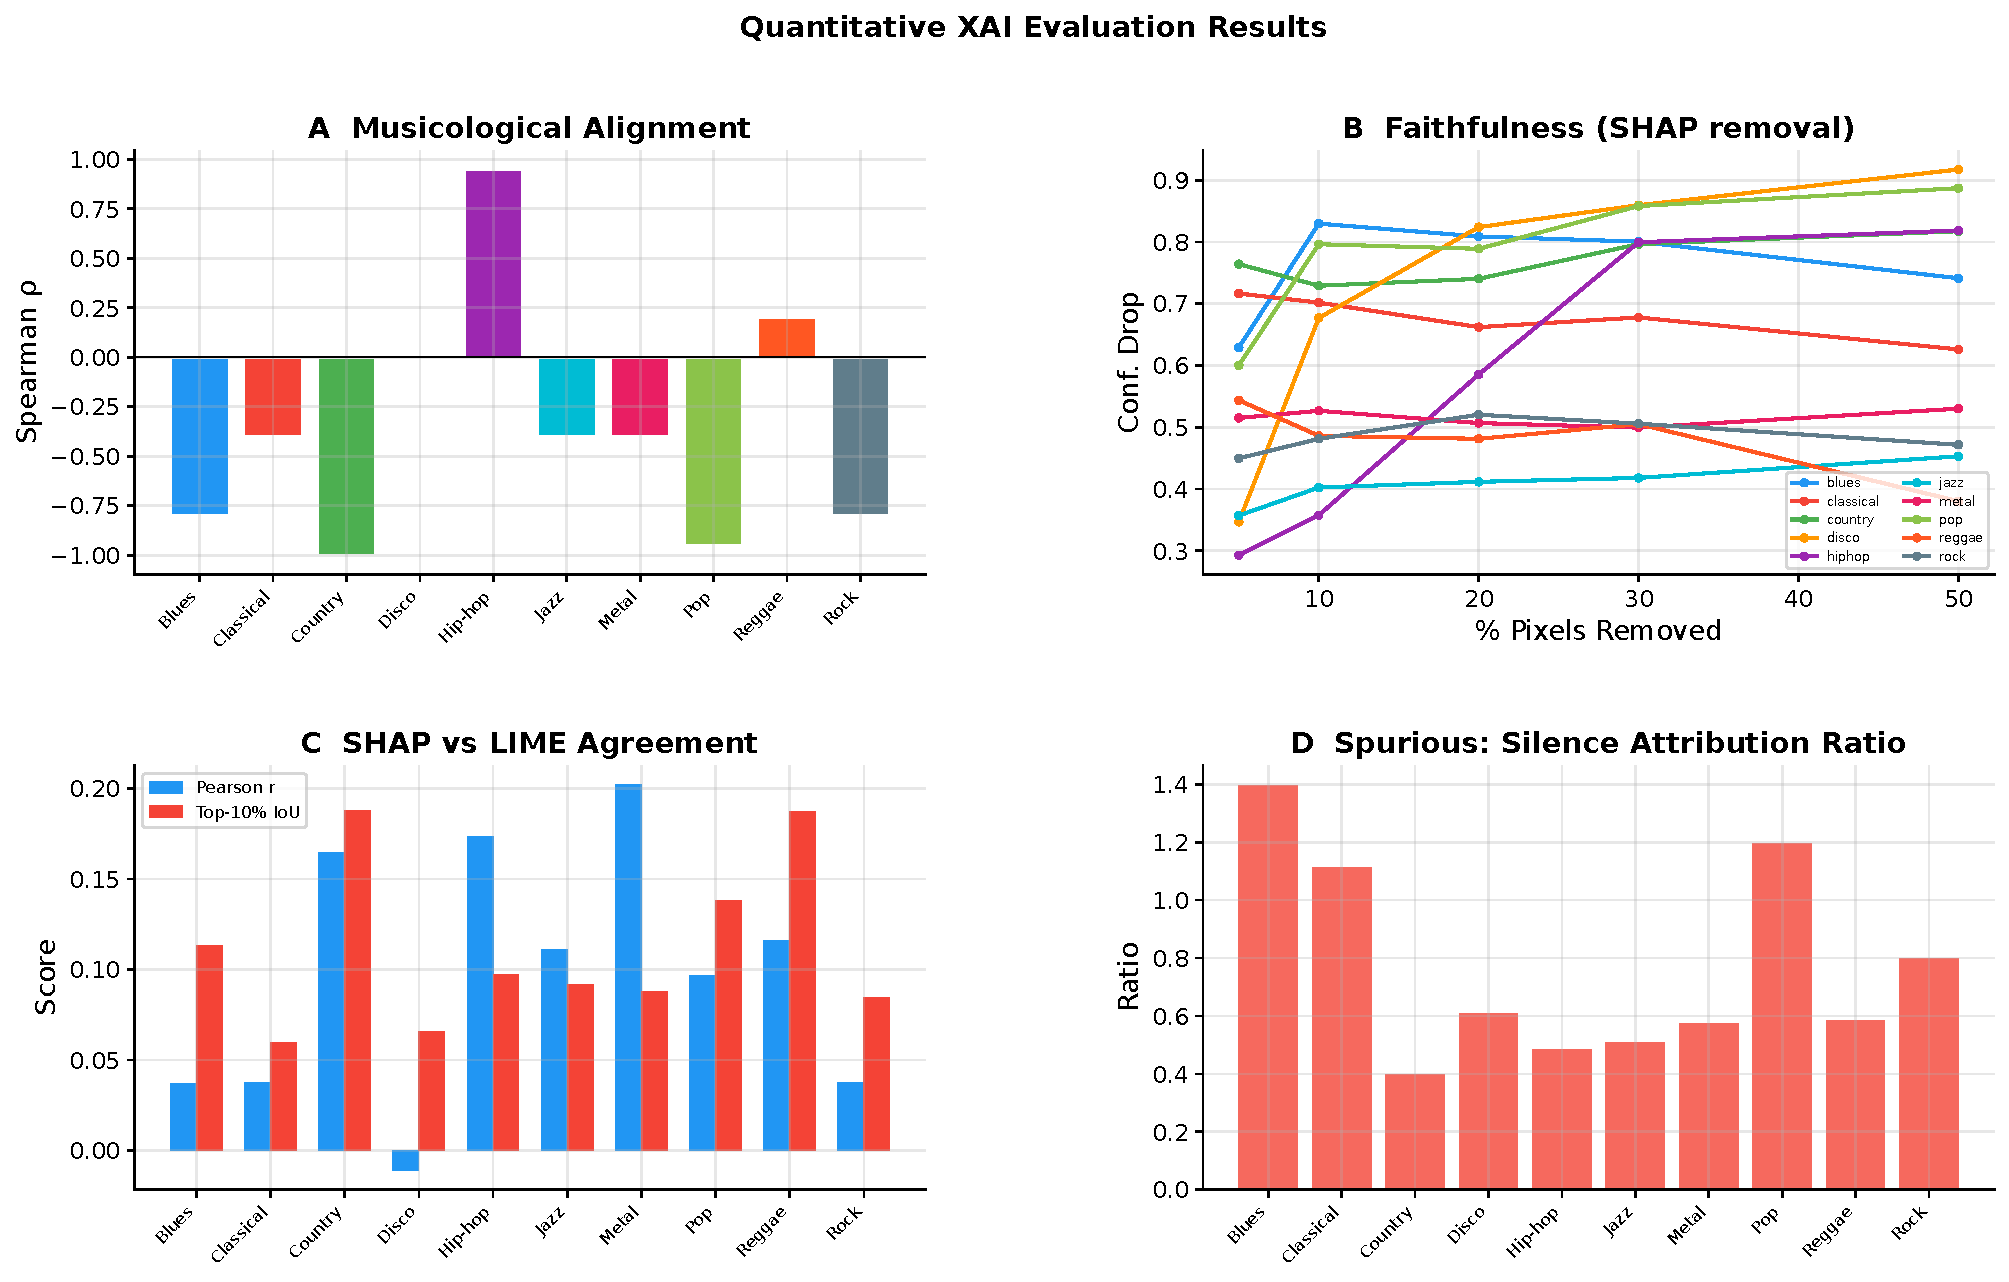
\includegraphics[alt={Four-panel figure showing musicological alignment, faithfulness curves, SHAP-LIME agreement, and spurious correlation results},width=0.98\textwidth]{FINAL_02_quantitative_panel.pdf}
  \caption{Quantitative XAI evaluation results. (A) Musicological alignment (Spearman $\rho$) per genre. (B) Faithfulness curves: prediction confidence drop under progressive SHAP-pixel masking. (C) SHAP\,vs.\,LIME agreement (Pearson $r$ and top-10\% IoU). (D) Spurious correlation: silence-to-high-energy SHAP attribution ratio.}
  \label{fig:quantitative_panel}
\end{figure*}

\subsection{Faithfulness evaluation}\label{subsec:faithfulness}

Faithfulness curves for all genres are presented in \figref{fig:faithfulness}. Masking the top 5\% of SHAP-identified pixels produces confidence drops ranging from 29\% (hip-hop) to 76\% (classical), confirming that SHAP identifies genuinely decision-critical regions. At the 50\% masking level, all genres show substantial confidence degradation.

\begin{figure*}[!t]
  \centering
  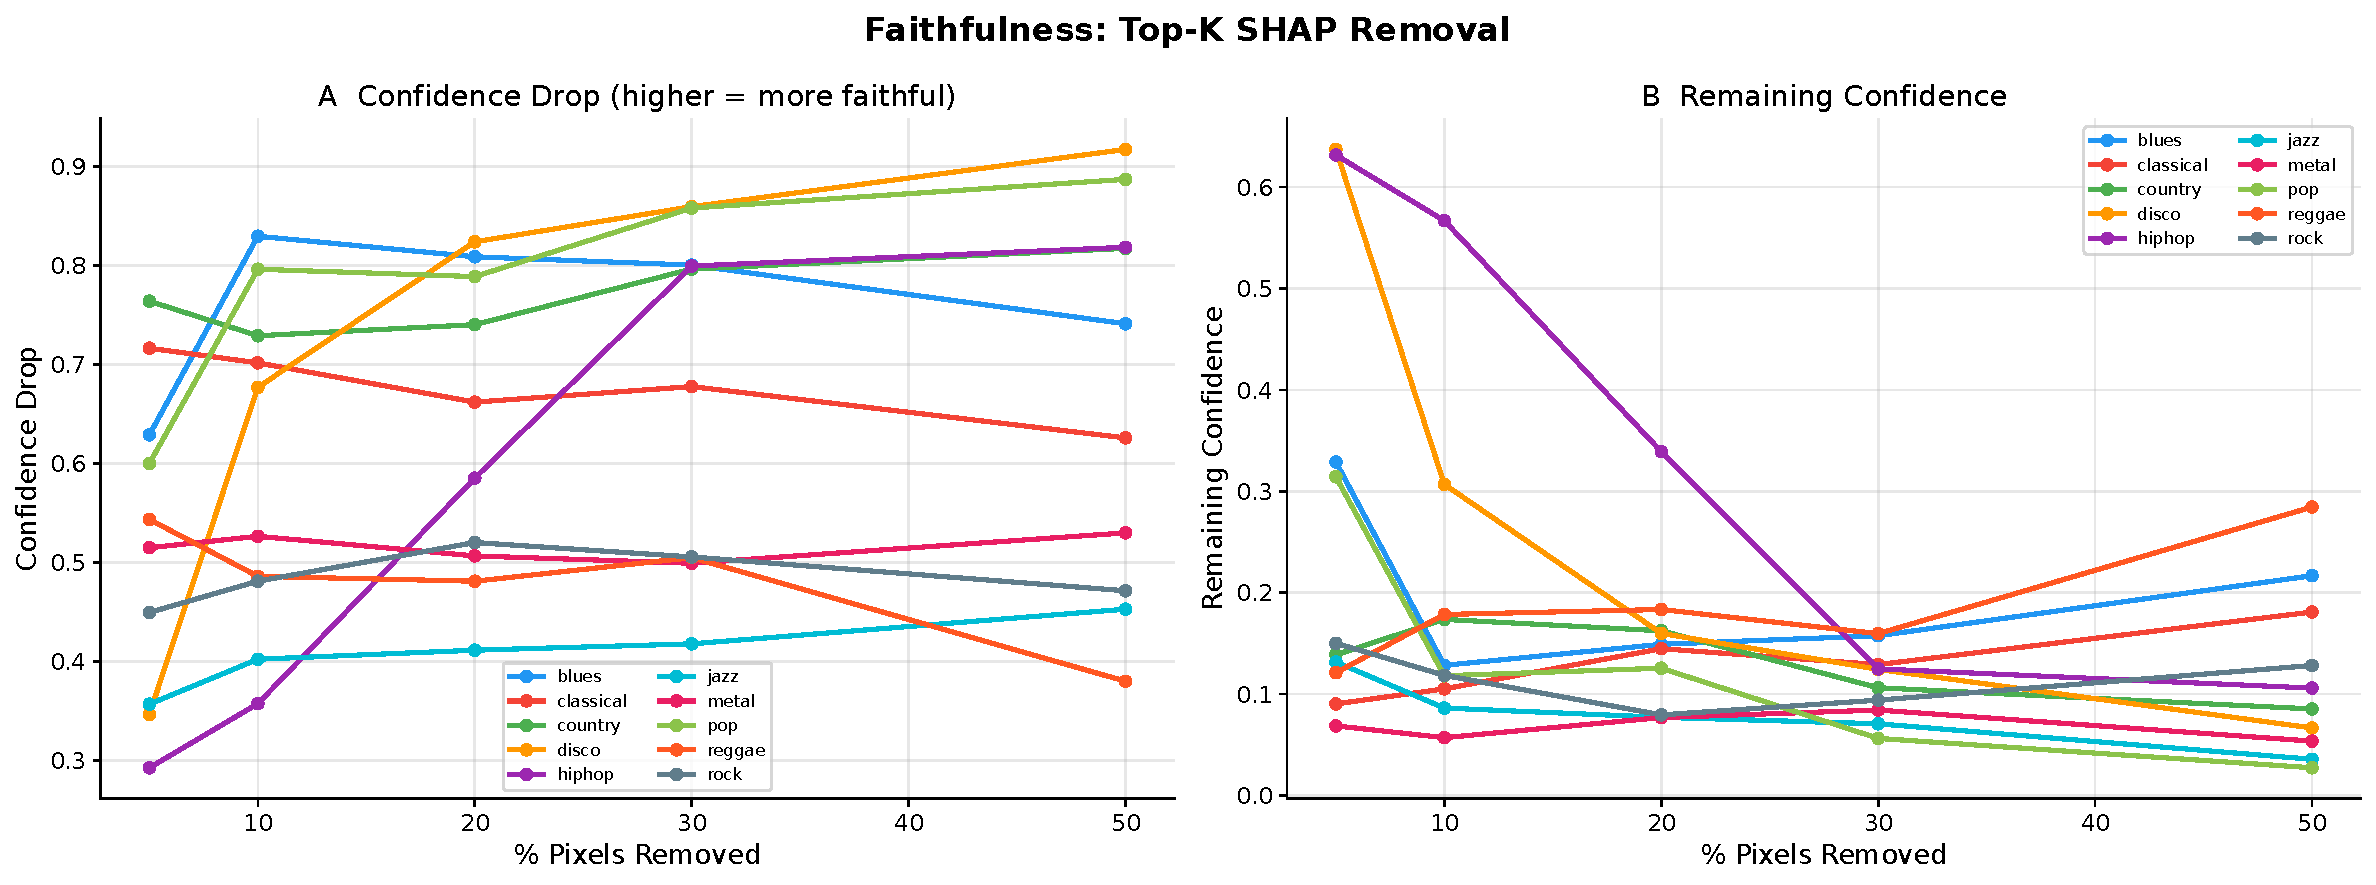
\includegraphics[alt={Line plots showing confidence drop as top SHAP pixels are progressively masked},width=0.95\textwidth]{05_faithfulness_curves.pdf}
  \caption{Faithfulness evaluation: prediction confidence drop as progressive fractions of the top-SHAP pixels are masked. Steeper curves indicate more faithful explanations.}
  \label{fig:faithfulness}
\end{figure*}

Disco (0.917) and pop (0.887) exhibit the highest faithfulness, indicating highly localised decision strategies. Reggae (0.380) shows the lowest faithfulness, suggesting the model relies on diffuse, distributed spectral cues rather than localised features for this genre.

\subsection{Music-informed spectral alignment}\label{subsec:alignment}

The Spearman correlation between observed SHAP band rankings and musicological expectations is shown in \figref{fig:alignment_fma} (panel A). The results reveal a striking genre-dependent pattern:

\textbf{Hip-hop} shows near-perfect positive alignment ($\rho = 0.95$): attribution concentrates in sub-bass and bass bands, consistent with well-known low-frequency emphasis in many hip-hop productions.

\textbf{Country} ($\rho = -1.0$) and \textbf{pop} ($\rho = -0.95$) exhibit near-perfect \textit{inverse} alignment. In isolation, this does not prove artifact use, but combined with elevated silence attribution ratios it is consistent with non-musical shortcut cues contributing to these predictions.

The remaining genres fall along a spectrum between these extremes, with reggae showing weak positive alignment ($\rho = 0.20$) and blues/rock showing substantial inverse tendencies ($\rho = -0.80$).

To reduce dependence on hand-crafted priors alone, we also compared SHAP band rankings against empirical GTZAN band profiles computed directly from the test audio. This empirical cross-check shows moderate positive agreement overall (mean $\rho \approx 0.38$ across genres), with substantial genre variation. We therefore treat prior-based and empirical alignment as complementary signals rather than interchangeable ground truths.

\subsection{Cross-dataset spectral profile check (FMA-small)}\label{subsec:fma_check}

To test whether the empirical band-profile patterns are specific to GTZAN, we ran a cross-dataset check on FMA-small \cite{Defferrard2017}. Using the same mel pipeline, we computed per-genre average band profiles on FMA-small (40 tracks per available mapped genre) and correlated them against GTZAN empirical profiles. The overlap is constrained by FMA-small labels: direct top-level matches provide hip-hop, pop, and rock, while explicit subgenre tags add metal and reggae. As shown in \figref{fig:alignment_fma} (panel B), all five comparable genres yield perfect rank-order agreement across the four bands ($\rho=1.0$ each), indicating that the broad spectral ordering learned for these classes is not unique to GTZAN.

\begin{figure*}[!t]
  \centering
  \begin{minipage}[t]{0.49\textwidth}
    \centering
    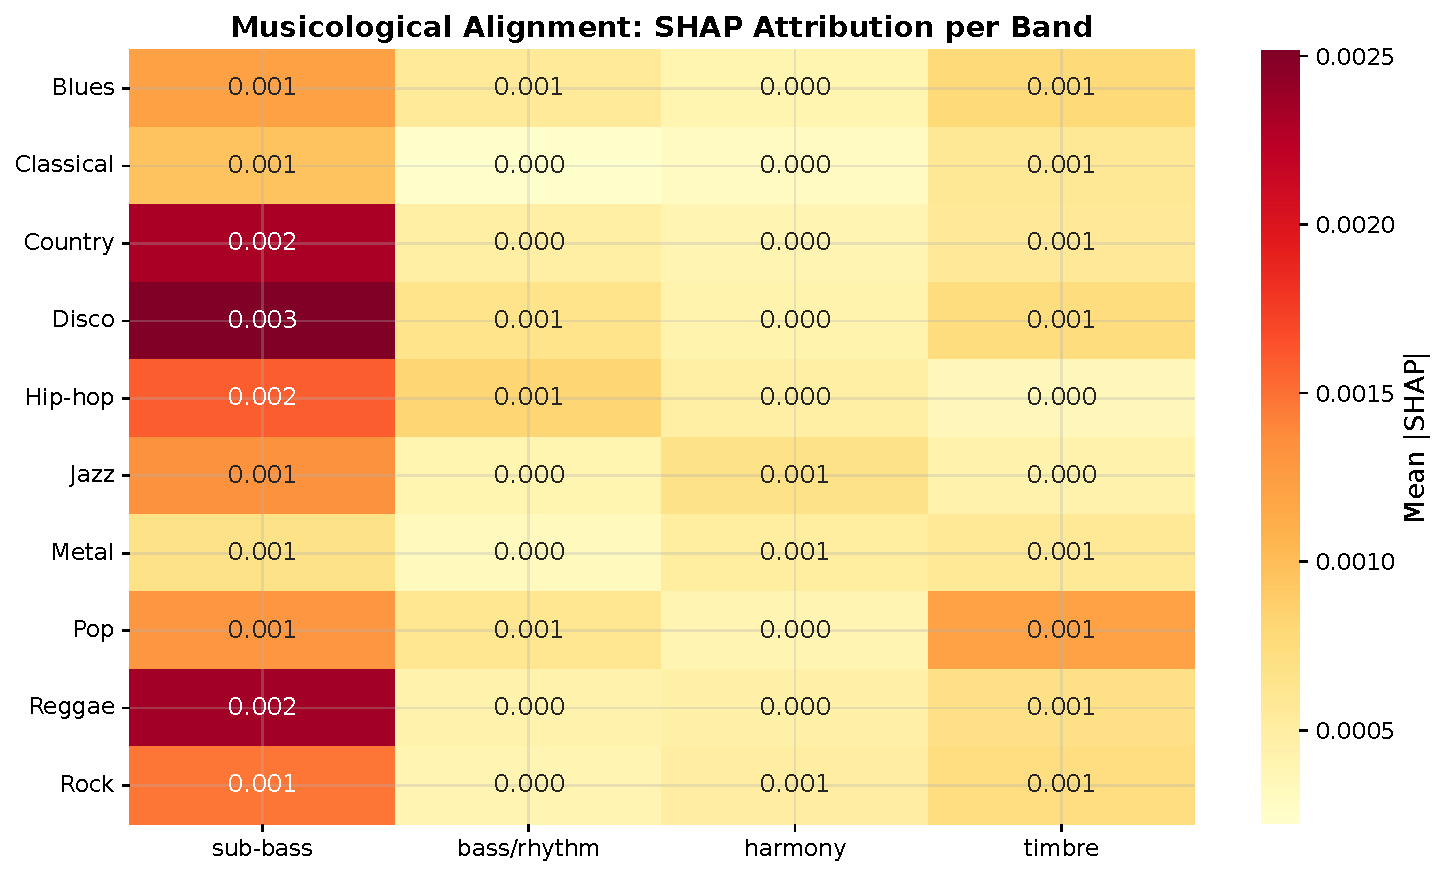
\includegraphics[alt={Bar chart showing musicological alignment scores per genre},width=\linewidth]{05_musicological_alignment.pdf}
  \end{minipage}\hfill
  \begin{minipage}[t]{0.49\textwidth}
    \centering
    \includegraphics[alt={Bar chart of Spearman correlation between GTZAN and FMA-small empirical band profiles for shared genres},width=\linewidth]{07_fma_gtzan_correlation.pdf}
  \end{minipage}
  \caption{Spectral-alignment analyses. (A) Music-informed spectral alignment scores by genre. Hip-hop shows strong positive alignment ($\rho = 0.95$), while country and pop show strong inverse alignment. (B) Cross-dataset check: Spearman correlation between GTZAN and FMA-small empirical band profiles for shared genres (hip-hop, metal, pop, reggae, rock).}
  \label{fig:alignment_fma}
\end{figure*}

\subsection{Inter-method agreement}\label{subsec:agreement}

Agreement between SHAP and LIME remains consistently low across genres, indicating substantial method-dependent explanation variance. As shown in \figref{fig:agreement}, Pearson correlations range from $r = -0.01$ (disco) to $r = 0.20$ (metal), and top-10\% IoU ranges from 6.0\% (classical) to 18.8\% (country).

\begin{figure*}[!t]
  \centering
  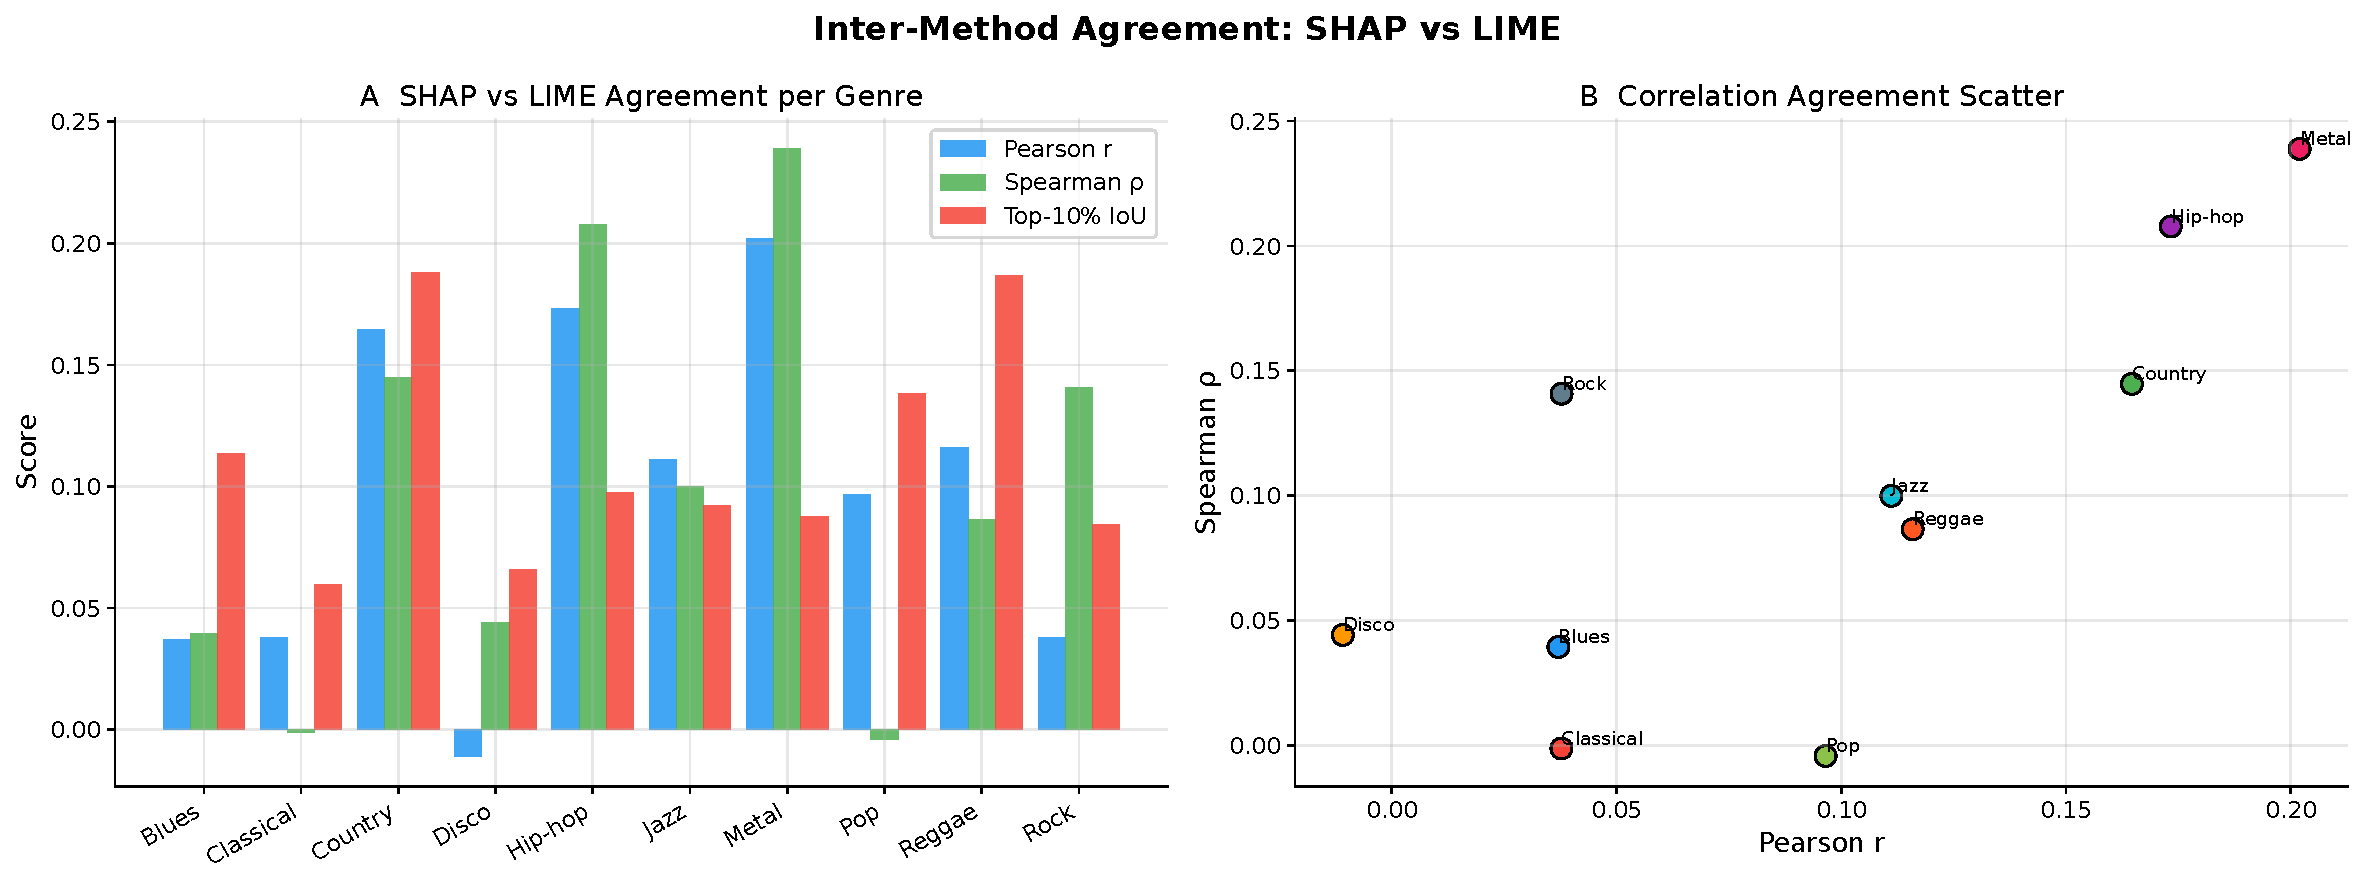
\includegraphics[alt={Heatmap showing SHAP vs LIME agreement metrics across genres},width=0.95\textwidth]{05_method_agreement.pdf}
  \caption{Inter-method agreement between SHAP and LIME. All three metrics (Pearson $r$, Spearman $\rho$, top-10\% IoU) show consistently low agreement across genres.}
  \label{fig:agreement}
\end{figure*}

This finding has significant implications. SHAP, operating at pixel granularity via gradient-based approximation, and LIME, operating at superpixel granularity via perturbation sampling, highlight fundamentally different aspects of the model's decision process. A practitioner using only SHAP would arrive at a different explanatory narrative than one using only LIME, even for the same prediction. This confirms and extends the disagreement problem identified in the general XAI literature \cite{Krishna2022} to the MIR domain.

\subsection{Spurious correlation detection}\label{subsec:spurious}

The spurious correlation analysis is presented in \figref{fig:spurious}, focusing on the silence attribution ratio.

\begin{figure*}[!t]
  \centering
  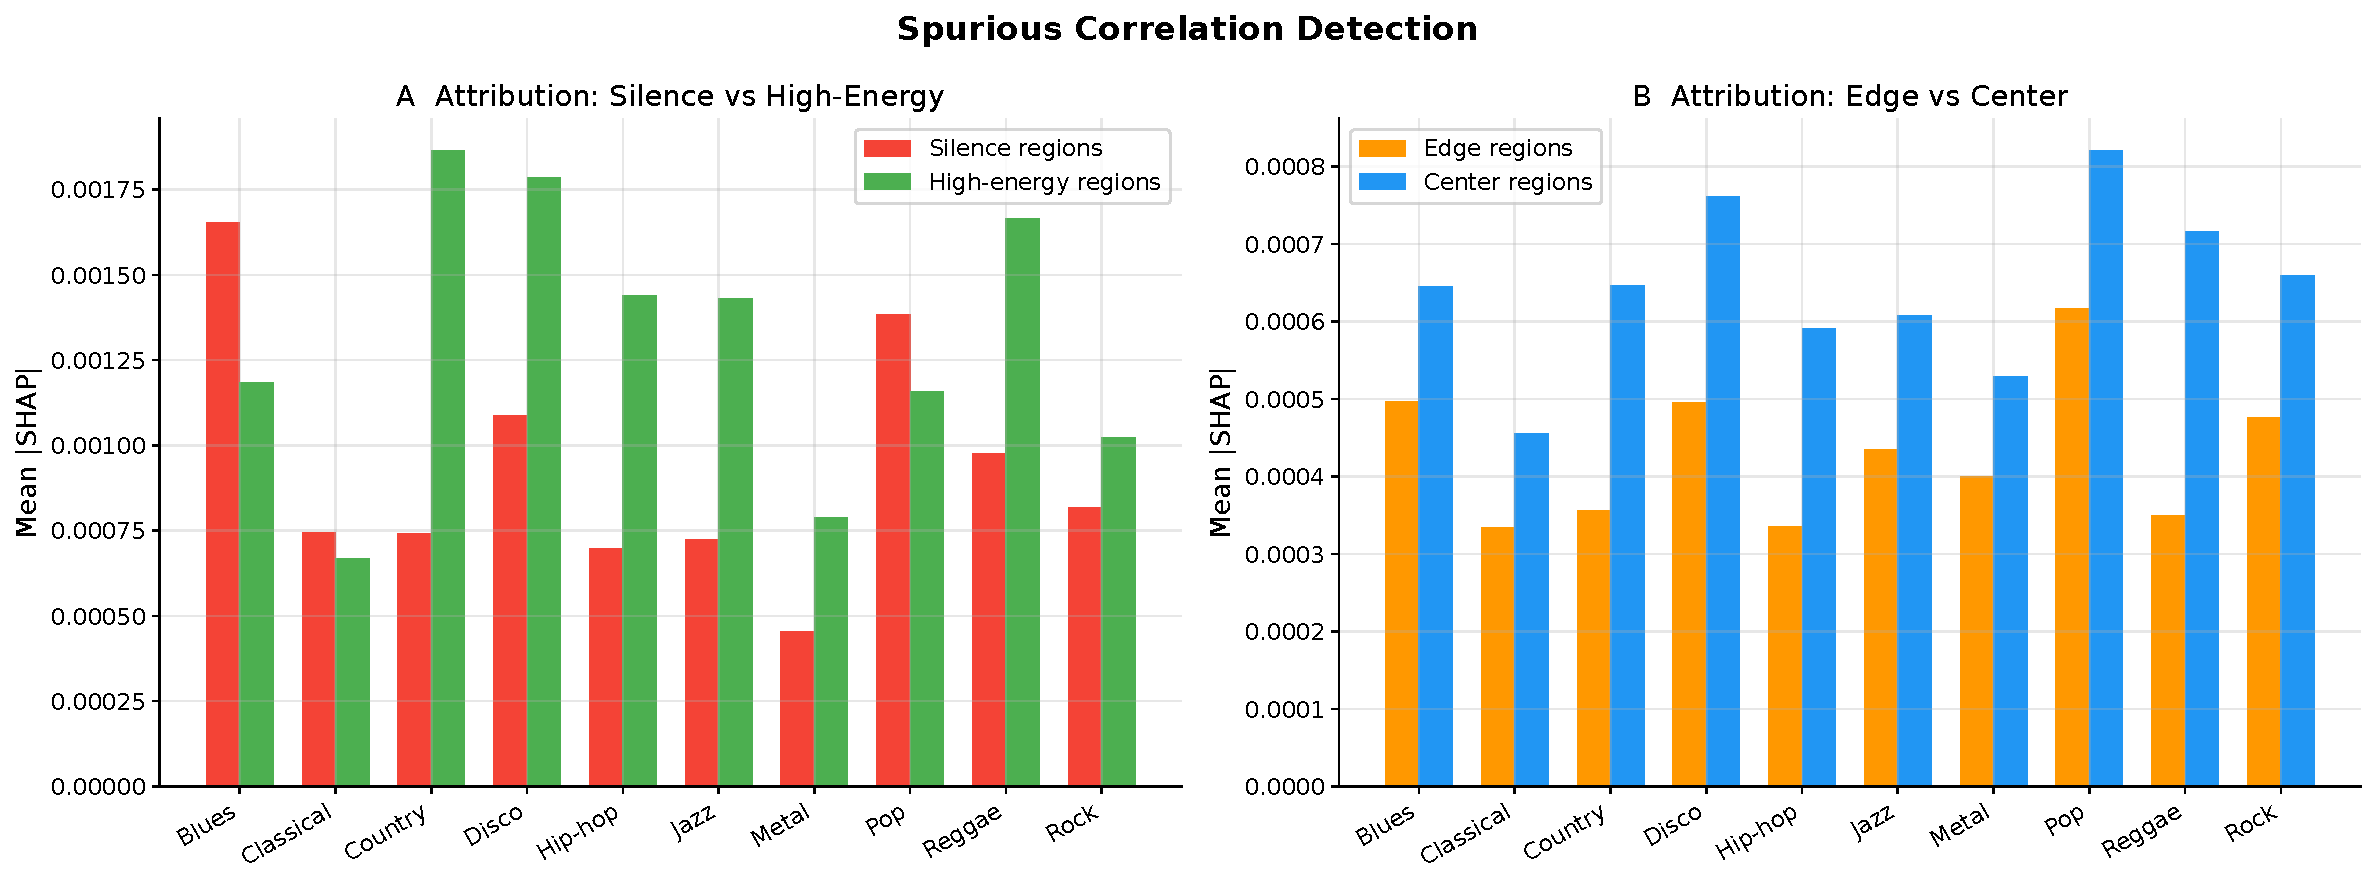
\includegraphics[alt={Bar chart comparing SHAP attribution in silence versus high-energy regions},width=0.95\textwidth]{05_spurious_correlation.pdf}
  \caption{Spurious correlation analysis: SHAP attribution ratio between silence and high-energy spectrogram regions. Blues and pop exceed 1.0, with classical also slightly above 1.0, indicating potential artifact sensitivity.}
  \label{fig:spurious}
\end{figure*}

\textbf{Blues} (ratio = 1.40) and \textbf{pop} (ratio = 1.20) show silence ratios exceeding 1.0, and \textbf{classical} is also marginally above 1.0 (ratio = 1.11). These patterns indicate increased sensitivity to low-energy bins relative to high-energy musical regions and are consistent with potential artifact reliance. One plausible explanation is that recording-noise floor or mastering characteristics contribute to classification in these genres.

For well-classified genres like hip-hop (ratio = 0.49), country (0.40), and jazz (0.51), attribution is concentrated more on high-energy content than silence.

\subsection{Transformer attention analysis}\label{subsec:attention}

CLS token attention heatmaps from the fine-tuned AST are displayed in \figref{fig:attention} for representative clips of each genre. The attention patterns complement the SHAP and LIME findings: genres with concentrated attention over specific time-frequency regions (e.g., hip-hop's low-frequency focus) generally correspond to higher musicological alignment scores, while genres with diffuse or edge-concentrated attention (e.g., blues) correspond to lower alignment.

\begin{figure*}[!t]
  \centering
  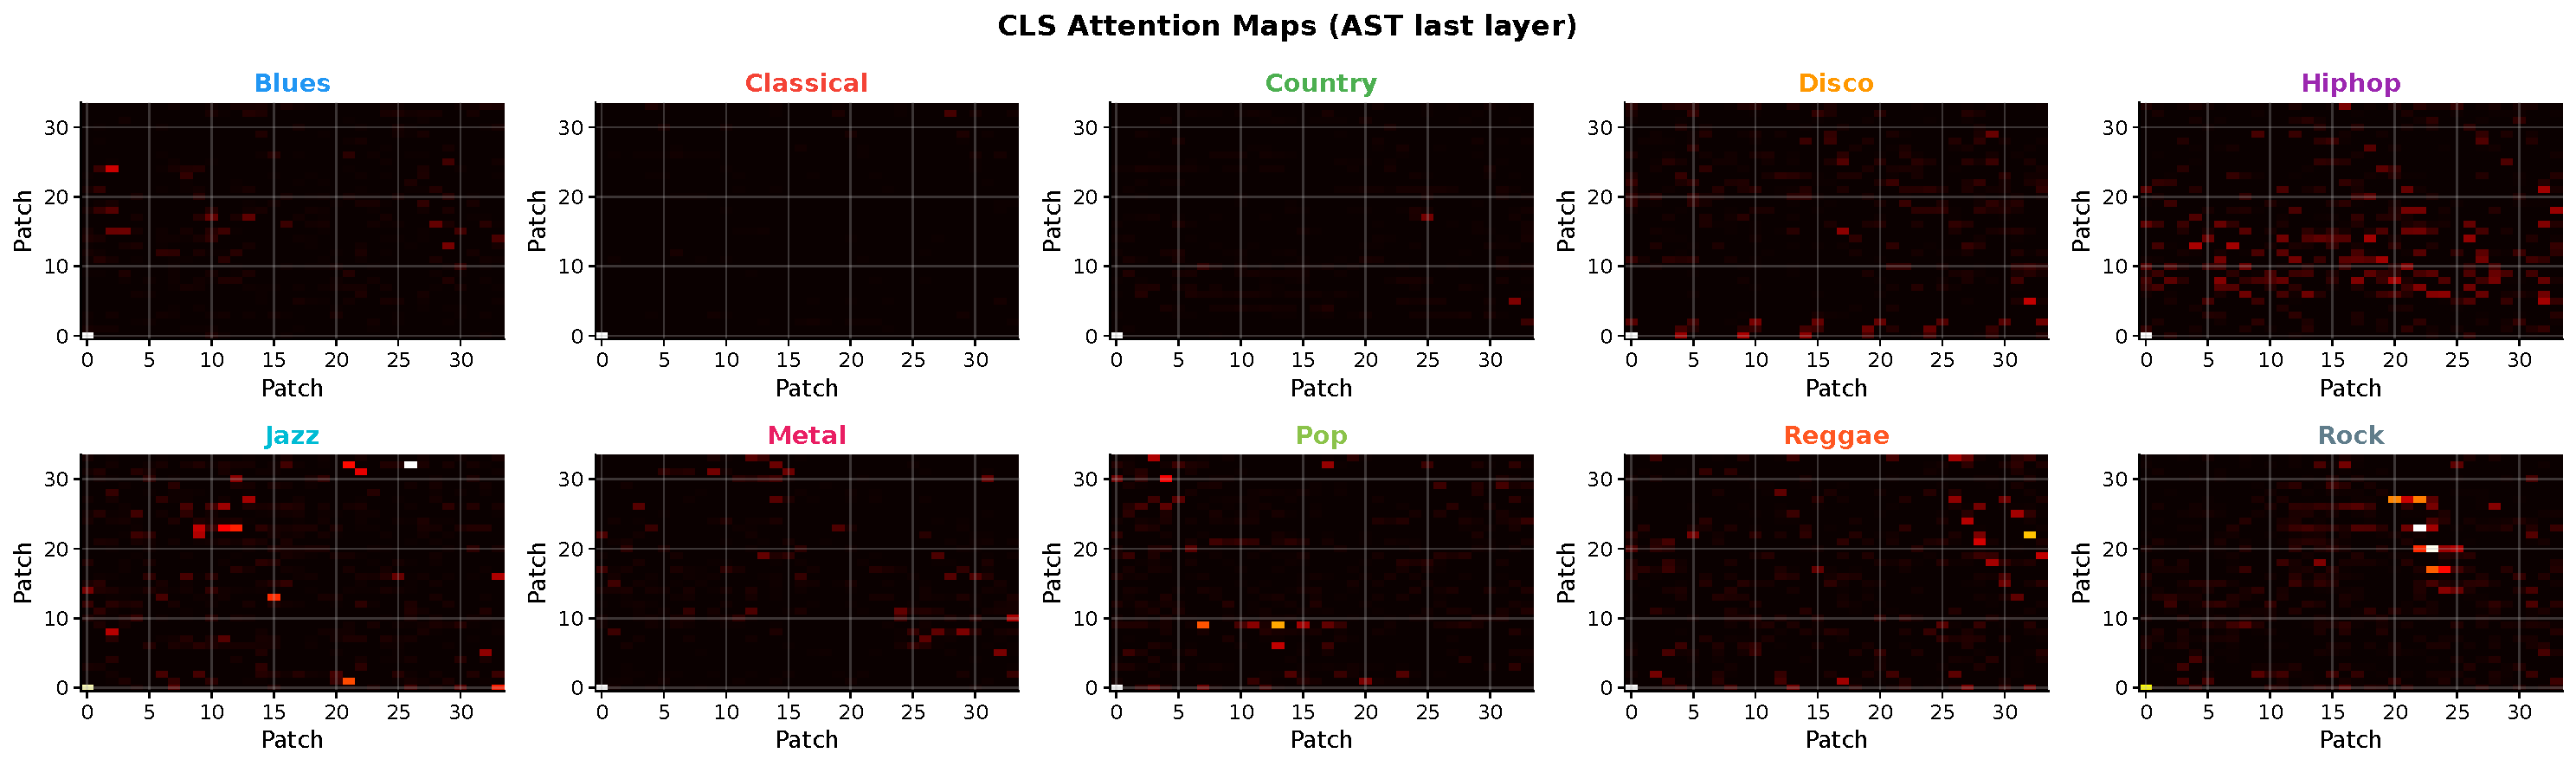
\includegraphics[alt={Gallery of AST CLS attention heatmaps for ten genres},width=0.95\textwidth]{06_attention_gallery.pdf}
  \caption{CLS token attention from the last self-attention layer of the fine-tuned AST, visualised over the input spectrogram for each genre. Brighter regions indicate higher attention weight.}
  \label{fig:attention}
\end{figure*}

\section{Discussion}\label{sec:discussion}

\subsection{A spectrum of musicological learning}

The results reveal that genre classifiers do not uniformly learn genuine musical features or uniformly exploit artifacts. Instead, each genre occupies a position along a spectrum. At one end, hip-hop classification shows attribution patterns consistent with expected low-frequency cues. At the other end, country and pop show inverse alignment with the spectral prior and, for pop, elevated silence attribution, suggesting increased vulnerability to non-musical cues.

This genre-dependent behaviour likely reflects the interaction between genre-specific acoustic properties and GTZAN's dataset characteristics. Hip-hop's spectral signature, dominated by low-frequency 808-style bass and drum machine patterns, is highly distinctive and consistent across recordings regardless of recording quality. In contrast, country and pop tracks in GTZAN may share less distinctive spectral signatures, leading the model to rely on secondary cues introduced by the dataset's construction.

\subsection{The disagreement problem in MIR}

The finding that SHAP and LIME produce low-agreement explanations (Pearson $r = 0.04$--$0.20$) has practical implications for MIR researchers and practitioners. If one were to diagnose model behaviour using only SHAP, one would identify fine-grained spectral regions as important. Using only LIME, one would identify broader contiguous regions, potentially suggesting different musical features as salient. This disagreement arises from methodological differences: SHAP computes pixel-level Shapley values via gradient-based approximation, while LIME perturbs superpixel-scale regions and fits a local linear model.

This disagreement is not a deficiency of either method alone, but rather a fundamental property of trying to explain complex, nonlinear decisions through simpler approximations. Each method captures a different facet of the model's decision surface. This finding supports the principle of \textit{multi-method triangulation}: explanations should be sought from diverse methods, and only conclusions supported by convergent evidence across methods should be treated as robust.

\subsection{Implications for dataset design}

The spurious correlation analysis provides quantitative evidence consistent with concerns raised by Sturm \cite{sturm2013gtzan, Sturm2014} about GTZAN. Elevated silence attribution in blues and pop indicates that recording-related cues may influence decisions. This implication extends beyond GTZAN: any music dataset with genre-correlated recording conditions risks shortcut learning.

Future dataset construction should incorporate: (1) recording-quality normalisation across genres; (2) explicit artist-disjoint train/test splits; and (3) routine XAI-based auditing of trained models to detect spurious feature reliance before deployment.

\subsection{Limitations}

Several limitations should be acknowledged when interpreting these results. The spectral-alignment analysis is intentionally simplified to broad frequency bands. This choice makes the metric transparent and reproducible, but it cannot represent important musical structure such as rhythmic patterning, harmonic progression, instrumentation, or production context. For this reason, alignment scores should be interpreted as coarse indicators of spectral emphasis rather than complete measures of ``musicological correctness.''

The cross-dataset analysis is also limited in scope by label availability in FMA-small. Under the official FMA-small subset and metadata, five GTZAN-comparable classes are supported with explicit mappings (hip-hop, metal, pop, reggae, rock) \cite{Defferrard2017}, whereas blues, classical, country, disco, and jazz are not represented with sufficient label support for this protocol. The five-class evaluation is therefore a constraint imposed by the external dataset, not a selective subset chosen after observing results. Consequently, the replication result should be interpreted as partial external validation. A stronger follow-up would evaluate the same framework on corpora with full label overlap and artist-disjoint splits.

Dataset and model constraints further bound the conclusions. Although known faulty GTZAN clips were excluded, residual artist and recording-condition effects may still remain \cite{Flexer2007}. In addition, the CNN used here was selected for interpretability and controlled attribution analysis, not for state-of-the-art accuracy. More expressive backbones may produce different attribution distributions and different levels of method agreement. Finally, AST attention is included as supporting qualitative evidence, but attention weights are not guaranteed to be causal explanations \cite{Jain2019}; the primary quantitative claims therefore rely on SHAP/LIME-based analyses and intervention tests.

Two method-specific limitations are also important. First, LIME explanations are produced with SLIC superpixels on spectrograms, and we did not run a dedicated segmentation ablation (e.g., alternative time-frequency partitioning) to test how sensitive conclusions are to this design choice. Second, we did not run saliency randomization sanity checks of the type proposed by Adebayo et~al.\ \cite{Adebayo2018}; adding these checks would strengthen claims about method reliability. Relatedly, faithfulness curves are constructed from SHAP-ranked masking, so they primarily validate SHAP-selected regions; extending the same perturbation protocol to LIME-defined regions is a useful next step to reduce method-centric evaluation bias.

\section{Conclusion}\label{sec:conclusion}

This work began from a simple but important question for modern MIR: when benchmark accuracy is high, what has the model actually learned? To answer this, we moved beyond aggregate performance reporting and conducted a systematic explainability study of genre classification on GTZAN. We combined SHAP, LIME, and auxiliary AST attention within one quantitative framework. The analysis jointly evaluated spectral-prior alignment, faithfulness under perturbation, inter-method agreement, and artifact-sensitive attribution behaviour.

Taken together, the results support three central conclusions. First, learned decision strategies are genre-dependent rather than uniform: some classes show attributions consistent with expected musical cues, while others show patterns compatible with shortcut usage. Second, explanation method choice materially affects interpretation: SHAP and LIME show persistently low agreement, which means single-method interpretation can produce unstable narratives. Third, quantitative artifact diagnostics, including silence-focused attribution ratios, provide practical signals for identifying classes at higher risk of relying on non-musical cues.

The contribution is both methodological and empirical. Methodologically, the paper provides a reproducible template for moving from qualitative saliency inspection to triangulated, metric-backed explanation analysis in MIR. Empirically, it reinforces long-standing concerns about dataset-induced shortcuts in GTZAN and also shows, through an FMA-small cross-dataset band-profile check, that key spectral rank patterns for shared genres replicate outside GTZAN. Overall, these findings support treating explainability as a core evaluation axis alongside accuracy, especially when models may be deployed beyond benchmark conditions.
To support transparency and reuse, the code, trained models, and experimental outputs are provided in an anonymised repository for review. The workflow covers data preparation, model training, explanation generation, quantitative evaluation, and cross-dataset checking so that the reported results can be independently reproduced. The GTZAN dataset is publicly available \cite{Tzanetakis2002}.

% Ethics Statement
\section{Ethics Statement}

This research uses the publicly available GTZAN dataset \cite{Tzanetakis2002}, which contains short excerpts of commercially released music used under fair use for non-commercial research. No human subjects were involved.

\FloatBarrier
\bibliography{references}

\end{document}
